\documentclass[a4paper,fleqn]{cas-sc}
\usepackage{fontspec}
\setmainfont{Nimbus Roman}[SmallCapsFont={Nimbus Roman}]
\setsansfont{Nimbus Sans}
\setmonofont{Nimbus Mono PS}
\usepackage[authoryear]{natbib}
\usepackage{amsmath,amssymb}
\usepackage{graphicx}
\usepackage{tikz}
\usetikzlibrary{positioning,fit,arrows.meta}
\usepackage{booktabs}
\usepackage{array}
\usepackage{float}
\usepackage{xcolor}
\usepackage{microtype}
\microtypesetup{expansion=false}
\IfFileExists{xurl.sty}{\usepackage{xurl}}{\usepackage{url}}
\setlength{\emergencystretch}{3em}
\floatstyle{ruled}
\newfloat{algorithm}{tbp}{loa}
\floatname{algorithm}{Алгоритм}
\floatstyle{plain}
\restylefloat{figure}
\restylefloat{table}
\newtheorem{proposition}{Твердження}
\newtheorem{corollary}{Наслідок}
\newdefinition{remark}{Зауваження}
\newproof{proof}{Доведення}
\newcommand{\ibar}{\bar{y}}
\newcommand{\sbar}{\bar{s}}
\newcommand{\Exp}{\mathrm{Exp}}
\newcommand{\Full}{\textup{\textsc{Full}}}
\newcommand{\TS}{\textup{\textsc{TwoScale}}}
\newcommand{\ind}{\mathbf{1}}
\newcommand{\eW}{e_{W}}

\renewcommand{\figurename}{Рисунок}
\renewcommand{\tablename}{Таблиця}
\renewcommand{\refname}{Література}
\RenewDocumentCommand{\keywordtitle}{}{Ключові слова}
\AtBeginDocument{
\newlabel{app:clique}{{A}{25}{}{}{}}
\newlabel{app:floor}{{B}{27}{}{}{}}
\newlabel{app:repro}{{C}{28}{}{}{}}
\newlabel{sec:discussion}{{7}{22}{}{}{}}
\newlabel{sec:res_descriptor}{{6.6}{20}{}{}{}}
\newlabel{sec:results}{{6}{15}{}{}{}}
\newlabel{tab:verification}{{3}{26}{}{}{}}
}
\begin{document}
\let\WriteBookmarks\relax
\shorttitle{Двомасштабне стохастичне моделювання з агрегованим міжспільнотним зв'язком}
\shortauthors{Y. Kuryliak and M.T.M. Emmerich}

\title[mode=title]{Двомасштабне стохастичне моделювання епідемій у мережах спільнот з агрегованим міжспільнотним зв'язком}

\author[1]{Yulian Kuryliak}[orcid=0000-0002-6600-2637]
\cormark[1]
\ead{yulian.a.kuryliak@lpnu.ua}
\affiliation[1]{organization={Інститут комп'ютерних наук та інформаційних технологій, Національний університет ``Львівська політехніка''},
            addressline={вул. Степана Бандери, 12},
            city={Львів},
            postcode={79000},
            country={Україна}}

\author[2]{Michael T. M. Emmerich}[orcid=0000-0002-7342-2090]
\ead{michael.t.m.emmerich@jyu.fi}
\affiliation[2]{organization={Факультет інформаційних технологій, Університет Ювяскюля},
            addressline={P.O. Box 35 (Agora)},
            city={Ювяскюля},
            postcode={FI-40014},
            country={Фінляндія}}

\cortext[1]{Автор для листування}


% Попередня анотація; розділи з результатами ще не включено.
\begin{abstract}[Анотація]
Епідемічні моделі часто поєднують докладні контактні мережі всередині спільнот із загальними даними про зв'язки між ними. Ми описуємо двомасштабний симулятор для такої ситуації. Кожна спільнота має локальний симулятор Gillespie, а макрорівень генерує міжспільнотні зараження за агрегованими інтенсивностями та вибирає їхні цілі рівномірно серед сприйнятливих вузлів. Ми описуємо локальні годинники, правило імпорту й синхронізацію через фіксовані часові інтервали. Окремо розглядаємо ідеальний процес із точним визначенням часу подій: він моделює сурогатну мережу з рівномірними міжспільнотними зв’язками. Порівняння з повномережевим Gillespie досліджує, як це наближення змінює часи прибуття інфекції та їхні розподіли. Мета --- з'ясувати, коли агреговані зв'язки відтворюють потрібні показники, та пояснити джерела відмінностей.
\end{abstract}
\begin{keywords}
Стохастичне моделювання \sep Алгоритм Gillespie \sep Багатомасштабне моделювання \sep Мережі спільнот \sep Моделювання епідемій \sep Похибка наближення
\end{keywords}
\maketitle
% Простіший чорний текст розділів 1--3; основа — узгоджена parallel-версія.

\section{Вступ}
\label{sec:introduction}

Епідемія поширюється на кількох рівнях. Усередині спільноти зараження може залежати від конкретних контактів між людьми \citep{keeling2005,pastorsatorras2015,kiss2017}. Для зв'язків між спільнотами дані часто менш докладні: наприклад, відома лише кількість пасажирів, обсяг поїздок на роботу або загальна вага зв'язку між двома місцями \citep{balcan2009,barbosa2018human}. Тому потрібна модель, яка поєднує докладну контактну мережу всередині кожної спільноти із загальними даними про зв'язки між спільнотами.

Така ситуація виникає на практиці. Локальну контактну мережу можна спостерігати, відновлювати або генерувати за відомими характеристиками, зокрема кластеризацією та середньою довжиною найкоротших шляхів \citep{eubank2004,danon2011}. Натомість зв'язки між спільнотами можуть бути відомі лише з транспортних, міграційних даних, даних про поїздки на роботу чи даних мобільних операторів \citep{barbosa2018human,chang2021}. Вони дають загальну силу зв'язку, але не визначають людей, через яких інфекція може перейти між спільнотами. Отже, ми можемо знати вагу зв'язку, не знаючи конкретних вузлів-мостів та їхнього стану.

Якщо відомі всі контакти, епідемію можна описати неперервним марковським ланцюгом (CTMC) і точно моделювати методом Gillespie \citep{gillespie1977exact,gibson2000}. Є також ефективні методи для часових, великих і розріджених мереж \citep{vestergaard2015,kuryliak2025simulating}. Проте їм усе одно потрібні конкретні контакти, здатні передавати інфекцію. Метапопуляційні моделі використовують загальні потоки між спільнотами, але зазвичай замінюють і докладну локальну мережу кількостями людей у різних станах \citep{colizza2007reaction,colizza2008,balcan2010modeling,ajelli2010}. Наша задача лежить між цими двома випадками: зберегти випадкове поширення між окремими вузлами всередині спільнот, використовуючи лише загальні дані для зв'язків між ними.

Ідею двомасштабного симулятор представлено в попередній конференційній роботі \citep{kuryliak2025towards}. Для кожної спільноти він запускає окремий локальний симулятор. Макрорівень використовує поточні стани спільнот і ваги зв'язків, щоб генерувати зараження, які надходять з іншої спільноти. У цій статті ми докладно описуємо метод і досліджуємо його похибку. Зокрема, з'ясовуємо, що втрачається, коли справжні міжспільнотні ребра та їхні кінцеві вузли замінено загальною вагою зв'язку, а імпортоване зараження потрапляє на випадково вибраний сприйнятливий вузол.

Головне питання: коли такого агрегованого зв'язку достатньо для відтворення потрібної нам характеристики повномережевого CTMC? Ми досліджуємо часи прибуття інфекції, їхні розподіли та можливість передавання через справжні контакти. Близькі часи ще не гарантують можливого шляху
передавання: двомасштабна модель може заразити іншу спільноту, поки всі справжні вузли-мости в спільноті-
джерелі ще сприйнятливі. Для перевірки ми використовуємо синтетичні мережі, у яких відомі всі контакти.
Повний Gillespie отримує всю мережу, а двомасштабний метод — лише локальні мережі та загальні ваги
міжспільнотних зв’язків.

Стаття має чотири основні результати.
\begin{enumerate}
\item Описуємо, як працює симулятор: кожна спільнота моделюється окремо, а спільний планувальник визначає
зараження між ними. Пояснюємо, як він узгоджує локальні симулятори на часових інтервалах фіксованої довжини (Розділ~\ref{sec:method}, Алгоритм~\ref{alg:scheduler}).
\item Показуємо, яку мережу метод моделює точно. Ідеальний процес точний для \emph{сурогатної мережі з рівномірними міжспільнотними зв’язками}: між кожними двома зв’язаними спільнотами всі вузли однієї з’єднано з усіма вузлами іншої, а загальну вагу зв’язку розподілено порівну між цими парами (Твердження~\ref{prop:surrogate}). Далі ми визначаємо джерела похибки та аналізуємо один експорт інфекції (Твердження~\ref{prop:ordering}).
\item Ми порівнюємо двомасштабний метод із повномережевим моделюванням Gillespie для передавання інфекції в одну сусідню спільноту та її поширення вздовж ланцюга спільнот. Відмінності оцінюємо за відносним зсувом медіани часу першого зараження та відстанню Вассерштайна між розподілами цих часів.  (Розділи~\ref{sec:design} і~\ref*{sec:results}).
\item Ми пропонуємо емпіричний показник точності для наших тестів. Він порівнює розкид часів зараження всередині спільноти з типовим часом передавання через одне міжспільнотне ребро (Розділ~\ref*{sec:res_descriptor}).
\end{enumerate}

Ми розглядаємо динаміку «сприйнятливий--інфікований» (SI) на статичних синтетичних мережах і використовуємо один фіксований крок синхронізації. Розділ~\ref{sec:related} пояснює зв'язок із попередніми методами. Розділ~\ref{sec:method} описує симулятор. У Розділі~\ref{sec:analysis} пояснено, яку інформацію агрегований зв'язок зберігає та втрачає. Розділи~\ref{sec:design} і~\ref*{sec:results} містять експерименти та результати. У Розділі~\ref*{sec:discussion} обговорено застосування, обчислювальні витрати й обмеження.

\section{Пов'язані праці}
\label{sec:related}

\paragraph{Моделювання випадкових подій.}
Прямий метод Gillespie вибирає наступну подію та її час за поточними інтенсивностями подій \citep{gillespie1977exact}. Метод наступної реакції підтримує окремий годинник для кожної можливої події \citep{gibson2000}. Обидва методи точні для CTMC, який вони моделюють. Якщо інтенсивність змінюється з часом, її можна накопичувати до досягнення випадкового порога \citep{ethier1986}. \citet{anderson2007} використав цю ідею для систем зі змінними інтенсивностями та затримками. Наш макрогодинник працює за тією самою ідеєю, але його інтенсивність змінюється разом зі станами локальних епідемій. Мережеві симулятори можуть зменшувати обсяг роботи, оновлюючи лише інтенсивності, на які вплинула остання подія \citep{vestergaard2015,kuryliak2025simulating}. Наші локальні симулятори використовують реалізацію з \citet{kuryliak2025simulating}.

Деякі багатомасштабні методи прискорюють моделювання хімічних реакцій, наближено описуючи реакції, що відбуваються значно частіше за інші \citep{haseltine2002,cao2005slow}. Наш метод прибирає іншу інформацію. Він зберігає локальні зараження, але не знає, які саме міжспільнотні ребра зараз здатні передавати інфекцію. Попри цю відмінність, співвідношення швидкостей локального поширення та міжспільнотного передавання допомагає пояснити похибку.

\paragraph{Моделі з кількома спільнотами.}
Метапопуляційні моделі описують кожну підпопуляцію кількостями людей у різних станах і зв'язують підпопуляції потоками мобільності. Їх використовували для дослідження глобального поширення та умов проникнення інфекції \citep{colizza2007reaction,colizza2008,balcan2009,balcan2010modeling}. Докладні дані мобільності також можна поєднувати з локальними моделями передавання \citep{chang2021}. Агентні моделі, своєю чергою, представляють окремих людей у всій системі \citep{eubank2004,kerr2021}. \citet{ajelli2010} порівняли ці два підходи. Досліджуваний тут метод зберігає окремі вузли та контакти всередині спільноти, але замінює невідомі індивідуальні контакти між спільнотами одним агрегованим стохастичним зв'язком.

\paragraph{Два рівні перемішування та спільне моделювання.}
Деякі епідемічні моделі поєднують контакти в малих локальних групах із рівномірним перемішуванням на ширшому рівні \citep{ball1997}. Наша сурогатна мережа з рівномірними міжспільнотними зв’язками має подібну ідею, але рівномірне перемішування діє лише між зв'язаними парами спільнот, а його силу визначає загальна вага зв'язку.

Реалізація також має риси спільного моделювання (co-simulation). У ньому окремі симулятори підсистем рухаються вперед за спільною часовою сіткою та обмінюються обмеженим набором даних \citep{gomes2018cosim}. У нас цими підсистемами є локальні симулятори спільнот. Вони передають макрорівню кількості інфікованих і сприйнятливих вузлів. Макрорівень використовує ці дані, щоб згенерувати час міжспільнотного зараження та вибрати спільноту-одержувача й цільовий вузол. Отже, локальні симулятори можуть залишатися «чорними скриньками» для планувальника. У цій реалізації дані, якими вони обмінюються, використовуються для створення випадкових подій зараження.

\section{Метод двомасштабного моделювання}
\label{sec:method}

В експериментах використано одну реалізацію двомасштабного симулятора, для якої локальні симулятори обмінюються з планувальником макро рівня через фіксовані проміжки часу. Щоб зрозуміти її похибку, ми також розглядаємо процес із тими самими інтенсивностями, але з точним визначенням часу кожної події. Цей теоретичний опис називаємо \emph{ідеальним процесом}. Він дає змогу відокремити похибку заміни мережі від додаткової похибки часової сітки. Ідеальний процес точний для сурогатної мережі з рівномірними міжспільнотними зв’язками, визначеної далі; це не означає точності для початкової фізичної мережі. Нижче пояснимо еталонну модель, доступні дані та кроки реалізованого симулятора.

\subsection{Повномережева еталонна модель}
\label{sec:reference}

Нехай $G=(V,E)$ --- контактна мережа. Її вузли поділено на $M$ спільнот, які не перетинаються:
\begin{equation}
\label{eq:partition}
V=V_1\cup V_2\cup\cdots\cup V_M,
\qquad N_i=|V_i|.
\end{equation}
Тут $V_i$ --- множина вузлів спільноти $i$, а $N_i$ --- кількість її вузлів. Позначаємо через $E_{ii}$ контакти всередині спільноти $i$, а через $E_{ij}$ --- контакти від вузлів спільноти $i$ до вузлів спільноти $j$. Контакт представляємо як напрямлений канал передавання. Тому ненапрямлений контакт дає два канали --- по одному в кожному напрямку.

Кожен вузол є сприйнятливим ($S$), інфікованим ($I$) або видаленим ($R$). Повний стан мережі в час $t$ позначаємо $X(t)$, а стан спільноти $i$ --- $X_i(t)$. Множини сприйнятливих та інфікованих вузлів цієї спільноти позначаємо $S_i(t)$ та $I_i(t)$. Їхні кількості --- $s_i(t)$ та $y_i(t)$, а частки --- $\sbar_i(t)=s_i(t)/N_i$ та $\ibar_i(t)=y_i(t)/N_i$. Далі $x$ означає конкретний стан мережі; $x^{v:I}$ --- той самий стан після зараження вузла $v$, а $x^{u:R}$ --- після видалення вузла $u$.

Повна модель має два прості правила переходів між станами. Сприйнятливий вузол $v$ отримує інфекцію від кожного інфікованого сусіда $u$ з інтенсивністю $\beta_{uv}$. Інфікований вузол видаляється з інтенсивністю $\gamma$. Для вузлів у відповідних станах:
\begin{equation}
\label{eq:full_generator}
q_v(x)=\sum_{\substack{u:(u,v)\in E\\x_u=I}}\beta_{uv}
\quad (x_v=S),
\qquad r_u(x)=\gamma\quad (x_u=I).
\end{equation}
Тут $q_v$ --- сумарна інтенсивність зараження вузла $v$, а $r_u$ --- інтенсивність видалення вузла $u$. Для несприйнятливого вузла $q_v=0$; для неінфікованого вузла $r_u=0$. Інтенсивність визначає частоту події: наприклад, за сталої інтенсивності $q$ середній час очікування дорівнює $1/q$.  Для міжспільнотного каналу записуємо $\beta_{uv}=\beta_{\mathrm{out}}w_{uv}$, де $w_{uv}$ --- вага контакту. Точне моделювання цих повномережевих інтенсивностей позначаємо \Full{}. Усі експерименти в статті мають динаміку SI, тобто $\gamma=0$.

Час переходу між станами є експоненційним і визначається сумарною інтенсивністю всіх подій у поточному стані $x$, яка дорівнює
\[
a(x)=\sum_v q_v(x)+\sum_u r_u(x).
\]
Якщо $a(x)>0$, час до наступної події має експоненційний розподіл із параметром $a(x)$ і середнім $1/a(x)$.
Зараження вузла $v$ вибирається з імовірністю $q_v(x)/a(x)$, а видалення вузла $u$ --- з імовірністю $r_u(x)/a(x)$.
Після події інтенсивності перераховуються.
Якщо $a(x)=0$, подальших подій немає.

\subsection{Агрегований інтерфейс}
\label{sec:interface}

Двомасштабний симулятор \TS{} знає кожен локальний граф $G_i=(V_i,E_{ii})$ та його інтенсивності. Він не знає конкретних міжспільнотних каналів у $E_{ij}$. Для кожної напрямленої пари спільнот йому відома лише загальна вага:
\begin{equation}
\label{eq:weight}
W_{ij}=\sum_{(u,v)\in E_{ij}}w_{uv},\qquad i\neq j.
\end{equation}
Якщо всі ваги дорівнюють одиниці, $W_{ij}$ --- кількість каналів від $V_i$ до $V_j$. У прикладній задачі цю величину можна оцінити за транспортними, міграційними даними, даними мобільності або контактів. Макрорівень також отримує поточні кількості сприйнятливих та інфікованих вузлів від кожного локального симулятора. Він не знає, які вузли є кінцями справжніх міжспільнотних ребер. Основні відмінності наведено в Таблиці~\ref{tab:information}; Рисунок~\ref{fig:schematic} показує їх на схемі.

\begin{table}[tbp]
\color{black}\centering
\caption{\textcolor{black}{Дані та правила двох моделей. В усіх експериментах \TS{} вибирає цільовий вузол рівномірно серед сприйнятливих вузлів.}}
\label{tab:information}
\small
\begin{tabular}{>{\raggedright\arraybackslash}p{0.42\linewidth}>{\raggedright\arraybackslash}p{0.23\linewidth}>{\raggedright\arraybackslash}p{0.25\linewidth}}
\toprule
Дані або дія & \Full{} & \TS{}\\
\midrule
Локальні контакти, інтенсивності та стани вузлів & відомі & відомі локальним симуляторам\\
Конкретні міжспільнотні ребра та вузли-мости & відомі & невідомі\\
Загальна міжспільнотна вага $W_{ij}$ & отримана з ребер & задана безпосередньо\\
Інтенсивність міжспільнотного зараження & зі станів кінців справжніх ребер & з $\ibar_i$, $\sbar_j$ та $W_{ij}$\\
Цільовий вузол зараження & кінець ребра, яке передало інфекцію & сприйнятливий вузол, вибраний за правилом\\
Кількість можливих SI-заражень через набір каналів & не більше кількості каналів & не більше $s_j$ цільових заражень\\
\bottomrule
\end{tabular}
\end{table}

\begin{figure}[tbp]
\color{black}\centering
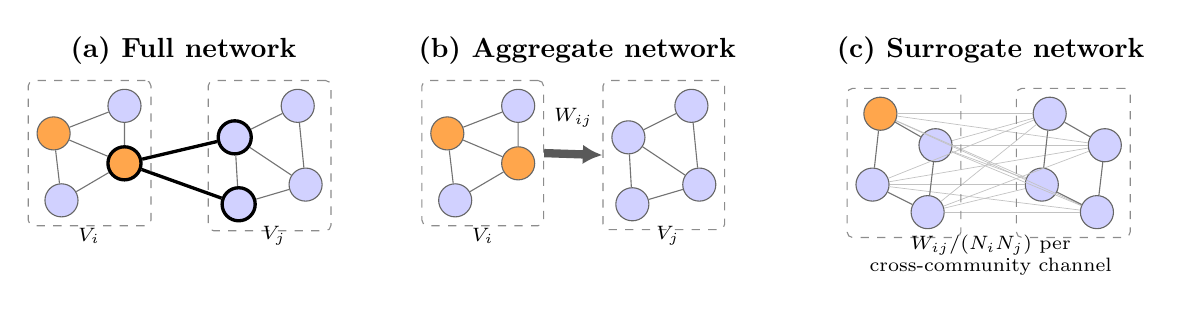
\begin{tikzpicture}[
  x=1cm,y=1cm,
  font=\scriptsize,
  >=Latex,
  person/.style={circle,draw=black!60,fill=blue!18,minimum size=4.2mm,inner sep=0pt},
  infected/.style={person,fill=orange!70},
  bridge/.style={person,very thick,draw=black},
  bridgeinf/.style={infected,very thick,draw=black},
  commbox/.style={draw=black!45,dashed,rounded corners=2pt,inner sep=3pt},
  macrobox/.style={draw=black!70,rounded corners=2pt,fill=black!5,align=center,inner sep=3pt},
  link/.style={draw=black!55},
  weak/.style={draw=black!24,line width=.25pt},
  flow/.style={-{Latex[length=1.7mm]},draw=black!65}
]
% (a) Full microscopic interface
\node[font=\bfseries] at (0,2.25) {(a) Full network};
\node[infected] (a1) at (-1.65,1.20) {};
\node[person]   (a2) at (-1.55,0.35) {};
\node[bridgeinf](a3) at (-0.75,0.82) {};
\node[person]   (a4) at (-0.75,1.55) {};
\node[bridge]   (b1) at (0.65,1.15) {};
\node[person]   (b2) at (1.45,1.55) {};
\node[person]   (b3) at (1.55,0.55) {};
\node[bridge]   (b4) at (0.70,0.30) {};
\draw[link] (a1)--(a2)--(a3)--(a1) (a1)--(a4)--(a3);
\draw[link] (b1)--(b2)--(b3)--(b4)--(b1) (b1)--(b3);
\draw[very thick] (a3)--(b1);
\draw[very thick] (a3)--(b4);
\node[commbox,fit=(a1)(a2)(a3)(a4)] {};
\node[commbox,fit=(b1)(b2)(b3)(b4)] {};
\node at (-1.2,-0.10) {$V_i$};
\node at (1.15,-0.10) {$V_j$};

% (b) Aggregate community network with local contacts retained
\node[font=\bfseries] at (5.0,2.25) {(b) Aggregate network};
\node[infected] (e1) at (3.35,1.20) {};
\node[person]   (e2) at (3.45,0.35) {};
\node[infected] (e3) at (4.25,0.82) {};
\node[person]   (e4) at (4.25,1.55) {};
\node[person]   (f1) at (5.65,1.15) {};
\node[person]   (f2) at (6.45,1.55) {};
\node[person]   (f3) at (6.55,0.55) {};
\node[person]   (f4) at (5.70,0.30) {};
\draw[link] (e1)--(e2)--(e3)--(e1) (e1)--(e4)--(e3);
\draw[link] (f1)--(f2)--(f3)--(f4)--(f1) (f1)--(f3);
\node[commbox,fit=(e1)(e2)(e3)(e4)] (agg_i) {};
\node[commbox,fit=(f1)(f2)(f3)(f4)] (agg_j) {};
\draw[-{Latex[length=2.5mm,width=2.5mm]},draw=black!65,line width=3pt]
      (agg_i.east) -- node[above=5pt,text=black] {$W_{ij}$} (agg_j.west);
\node at (3.8,-0.10) {$V_i$};
\node at (6.15,-0.10) {$V_j$};

% (c) Surrogate interface
\node[font=\bfseries] at (10.25,2.25) {(c) Surrogate network};
\node[infected] (c1) at (8.85,1.45) {};
\node[person]   (c2) at (8.75,0.55) {};
\node[person]   (c3) at (9.55,1.05) {};
\node[person]   (c4) at (9.45,0.20) {};
\node[person]   (d1) at (11.00,1.45) {};
\node[person]   (d2) at (10.90,0.55) {};
\node[person]   (d3) at (11.70,1.05) {};
\node[person]   (d4) at (11.60,0.20) {};
\foreach \u in {c1,c2,c3,c4}{\foreach \v in {d1,d2,d3,d4}{\draw[weak] (\u)--(\v);}}
\draw[link] (c1)--(c2)--(c4)--(c3)--(c1);
\draw[link] (d1)--(d2)--(d4)--(d3)--(d1);
\node[commbox,fit=(c1)(c2)(c3)(c4)] {};
\node[commbox,fit=(d1)(d2)(d3)(d4)] {};
\node[align=center] at (10.25,-0.35) {$W_{ij}/(N_iN_j)$ per\\cross-community channel};
\end{tikzpicture}
\caption{\textcolor{black}{Три подання зв'язку між спільнотами. (a) У повній мережі інфекція переходить лише через показані фізичні ребра та їхні вузли-мости. (b) Усередині кожної спільноти збережено вузли та локальні контакти. Окремі міжспільнотні контакти подано одним широким напрямленим ребром між $V_i$ та $V_j$ із загальною вагою $W_{ij}$. (c) Ідеальний двомасштабний процес еквівалентний процесу на сурогатній мережі з рівномірними міжспільнотними зв’язками: між кожними двома зв’язаними спільнотами всі напрямлені пари вузлів мають однакову вагу контакту. Загальна вага всіх цих зв'язків дорівнює $W_{ij}$. Помаранчеві вузли --- інфіковані, сині --- сприйнятливі.}}
\label{fig:schematic}
\end{figure}

\subsection{Локальні симулятори}
\label{sec:local}

Кожна спільнота має окремий симулятор Gillespie для свого графа $G_i$. Він застосовує інтенсивності зараження та видалення з~\eqref{eq:full_generator}, використовуючи лише локальні ребра $E_{ii}$. Реалізація оновлює лише ті інтенсивності, на які вплинула остання подія, як у \citet{kuryliak2025simulating}. Кожен локальний симулятор є незалежним і має власний потік випадкових чисел.

Макрорівень може просунути локальний симулятор до заданого часу. Симулятор виконує локальні події до цього моменту. Потім макрорівень може імпортувати інфекцію, змінивши стан вибраного сприйнятливого вузла на $I$. Це змінює локальні інтенсивності. Реалізація зберігає невикористану частину випадкового порога наступної локальної події та перераховує час очікування за новою сумарною інтенсивністю. 

Щоб перерахувати час наступної локальної події після імпорту, симулятор зберігає залишок випадкового порога. Нехай $E_{\mathrm{loc}}\sim\mathrm{Exp}(1)$ --- поріг,
згенерований після попередньої локальної події, а
$A_{\mathrm{loc}}$ --- інтеграл сумарної локальної
інтенсивності від тієї події до моменту імпорту.
Після імпорту сумарна локальна інтенсивність
дорівнює $a_{\mathrm{new}}$. Якщо $a_{\mathrm{new}}>0$,
залишковий час очікування становить
\[
\Delta t=
\frac{E_{\mathrm{loc}}-A_{\mathrm{loc}}}{a_{\mathrm{new}}}.
\]
Отже, імпорт змінює час очікування, але не сам випадковий
поріг. Якщо раніше відбудеться ще один імпорт, накопичену
інтенсивність оновлюють і час очікування знову
перераховують. Якщо $a_{\mathrm{new}}=0$, локальна подія
не може відбутися, доки інтенсивність не стане додатною.

Тип події та її вузол вибираються за оновленими інтенсивностями. Новий локальний поріг генерується лише тоді, коли збереженого порога немає. Кожен локальний годинник має власний поріг, окремий від макропорога, описаного в Розділі~\ref{sec:timing}. За заданих часів імпорту та цільових вузлів локальний симулятор виконує правила CTMC своєї мережі. Наближення виникає через спосіб генерування імпортів і вибору їхніх цільових вузлів.

\subsection{Макрорівень}
\label{sec:macro}

Макрорівень представляє спільноту її поточними частками вузлів, а напрямлений зв'язок --- вагою $W_{ij}$. Інтенсивність зараження зі спільноти $i$ до спільноти $j$:
\begin{equation}
\label{eq:macro_rate}
\lambda_{ij}(t)=\beta_{\mathrm{out}}W_{ij}\ibar_i(t)\sbar_j(t),
\qquad \Theta(t)=\sum_{i\neq j}\lambda_{ij}(t).
\end{equation}
Кожен множник має простий зміст. $\beta_{\mathrm{out}}W_{ij}$ задає загальну силу зв'язку; $\ibar_i$ --- частку інфікованих у спільноті-джерелі; $\sbar_j$ --- частку сприйнятливих у спільноті-одержувачі. Сума $\Theta$ --- інтенсивність будь-якого міжспільнотного зараження. Обчислення часу до наступної події, за умови що $\Theta$ змінна в часі, має певні особливості (див \ref{sec:timing}).

Коли така подія відбувається, спочатку вибирають спільноту-джерело та спільноту-одержувача $(i,j)$ з імовірністю $\lambda_{ij}/\Theta$. Потім у спільноті $j$ рівномірно вибирають один сприйнятливий вузол і заражають його. Якщо таких вузлів 20, кожен має імовірність $1/20$. Вибір не враховує справжні вузли-мости, оскільки агрегований інтерфейс їх не знає. У подальших формулах цю імовірність позначаємо $\Pi_{ij}(v\mid x)=1/s_j$ для $v\in S_j$, де $x$ --- поточний стан мережі. Отже, $\Pi$ просто позначає імовірність вибору конкретного сприйнятливого вузла. Інші правила можливі, якщо є інформація про вузли-мости. 

Ця агрегована інтенсивність загалом наближено описує передавання через справжні фізичні ребра. Для заданих кількостей вузлів у станах вона дорівнює очікуваній інтенсивності за рівномірного випадкового вибору кінців ребер, перш ніж враховано їхні конкретні ідентичності, стани та історію епідемії. Це не гарантує правильної інтенсивності для вже реалізованої епідемії на конкретних ребрах. Для рівномірного зв'язку «усі з усіма» вона є фактичною інтенсивністю, як пояснено в Розділі~\ref{sec:analysis}. 

\subsection{Час подій та синхронізація}
\label{sec:timing}

Після макроподії в час $t_0$ генеруємо випадковий поріг $E\sim\Exp(1)$: експоненційне випадкове число із сподіванням один. Починаючи з нуля, накопичуємо загальну інтенсивність $\Theta$:
\begin{equation}
\label{eq:hazard_integral}
A(t)=\int_{t_0}^{t}\Theta(s)\,ds,
\qquad A(t_0)=0.
\end{equation}
Наступна макроподія відбувається в перший момент
$t^\ast$, коли $A(t^\ast)=E$.


Інакше кажучи, площа під кривою інтенсивності зростає до випадкового порога. Якщо поріг не досягнуто, наступної макроподії немає. Це стандартний спосіб визначення часу події за накопиченою інтенсивністю \citep{ethier1986,anderson2007}. За сталої $\Theta$ час очікування дорівнює $E/\Theta$. Якщо згенерувати $E=-\ln U$, де $U$ рівномірно розподілене на $(0,1)$, отримуємо звичний час очікування Gillespie. Коли локальна подія змінює $\Theta$, зберігаємо той самий поріг і продовжуємо накопичення з новою інтенсивністю. Новий макропоріг генеруємо лише після макроподії. Точне визначення першого досягнення порога задає ідеальний процес; описаний нижче розрахунок на часовій сітці наближено визначає цей момент. У Розділі~\ref{sec:surrogate} показано, що ідеальний процес точний для сурогатної мережі з рівномірними міжспільнотними зв’язками.

Планувальник ділить час на інтервали довжини $\tau$.
На кожному інтервалі він наближено замінює змінну
макроінтенсивність її значенням у середині інтервалу. Нехай $A$ --- уже накопичена величина від попередньої макроподії. Для поточного інтервалу $[t,t_g)$ копіюємо кожен локальний симулятор разом зі станом генератора випадкових чисел і просуваємо копію до середини інтервалу. За копіями обчислюємо оцінку загальної макроінтенсивності $\Theta_{\mathrm{mid}}$. Оцінений приріст за залишок інтервалу дорівнює $\Theta_{\mathrm{mid}}(t_g-t)$. Якщо $A$ плюс цей приріст менше за $E$ (випадковий макропоріг), справжні симулятори просуваються до $t_g$. Інакше час події оцінюємо як
\begin{equation}
\label{eq:interpolation}
t^\ast=t+\frac{E-A}{\Theta_{\mathrm{mid}}}.
\end{equation}
Тут $E$ --- випадковий макропоріг, а $A$ --- уже накопичена до нього величина. Чисельник $E-A$ --- залишок до порога; ділення на оцінену інтенсивність дає залишковий час очікування. Наприклад, за $E=1$, $A=0.4$ та $\Theta_{\mathrm{mid}}=0.2$ оцінений час очікування дорівнює трьом одиницям часу. Планувальник просуває справжні симулятори до $t^\ast$, за їхніми станами в цей момент вибирає спільноту-джерело та спільноту-одержувача, вибирає сприйнятливий цільовий вузол і застосовує зараження. Повну послідовність наведено в Алгоритмі~\ref{alg:scheduler}.

\begin{algorithm}[tbp]
\color{black}
\caption{\textcolor{black}{Один запуск двомасштабного симулятора з узгодженням за часовою сіткою.}}
\label{alg:scheduler}
\small

\textbf{Вхід:} локальні графи $G_i$, ваги $W_{ij}$, інтенсивності, крок $\tau$, горизонт $T_{\mathrm{end}}$ та початковий стан.
\begin{enumerate}
\item Установити $t=0$ і $A=0$; згенерувати $E\sim\Exp(1)$.
\item Поки $t<T_{\mathrm{end}}$ й інфекція може поширюватися, встановити $t_g=\min(t+\tau,T_{\mathrm{end}})$ та обробити інтервал до $t_g$.
\item Скопіювати кожен локальний симулятор разом зі станом генератора випадкових чисел. Просунути копії до середини залишку інтервалу та обчислити $\Theta_{\mathrm{mid}}$ за~\eqref{eq:macro_rate}.
\item Якщо $A+\Theta_{\mathrm{mid}}(t_g-t)<E$, просунути справжні симулятори до $t_g$, додати цю величину до $A$, встановити $t=t_g$ і повернутися до кроку 2.
\item Інакше обчислити $t^\ast$ за~\eqref{eq:interpolation} та просунути справжні симулятори до $t^\ast$.
\item Вибрати $(i,j)$ з імовірністю $\lambda_{ij}(t^\ast)/\Theta(t^\ast)$. Рівномірно вибрати $v$ з $S_j(t^\ast)$ та імпортувати зараження у $v$. Оновити локальний симулятор одержувача, зберігаючи невикористаний експоненційний поріг і вибираючи локальну подію за новими інтенсивностями.
\item Установити $t=t^\ast$ і $A=0$, згенерувати нове $E\sim\Exp(1)$ та так само обробити залишок поточного інтервалу.
\end{enumerate}

\end{algorithm}

Копіювання станів генераторів випадкових чисел важливе: якщо до середини інтервалу не відбудеться імпорт, копія відтворить ту саму траєкторію, що й справжній симулятор. Оцінка середньої точки точна на інтервалі без локальних подій. Її похибка визначення часу та використання майбутнього стану не більш як на $\tau/2$ зникають зі зменшенням $\tau$ до нуля.

Часова сітка потрібна, оскільки планувальник працює з локальними симуляторами як із «чорними скриньками». Якщо вони також повідомляють часи наступних локальних подій, планувальник може об'єднати ці часи та точно накопичувати $\Theta$, яка стала між подіями. Такий подієвий варіант усуває чисельну похибку синхронізації. В експериментах цієї статті використано реалізований сітковий варіант із $\tau=1$.

\subsection{Обчислювальна структура та застосування}
\label{sec:cost}

\Full{} зберігає всі локальні та міжспільнотні канали, а обсяг роботи на одну подію зростає зі степенем вузла \citep{kuryliak2025simulating}. \TS{} зберігає локальні графи та матрицю загальних ваг розміру $M\times M$. У конференційній роботі обговорено таке скорочення даних про міжспільнотні контакти \citep{kuryliak2025towards}. Його значення залежить від задачі. Заміна багатьох індивідуальних міжспільнотних ребер однією вагою може зменшити обсяг збережених даних. Якщо таких ребер лише кілька, економія може бути малою; локальні графи все одно потрібно зберігати.

Окремі локальні симулятори також створюють можливість паралельного виконання. Коли планувальник визначив наступний цільовий час ($t_g$ або $t^\ast$), локальні симулятори можна незалежно просунути до цього самого часу. Копії для оцінки середньої точки також можна обробляти паралельно. Потім макрорівень має зібрати кількості вузлів і застосувати імпорт, якщо він запланований, перш ніж продовжувати. У досліджуваній реалізації локальні симулятори просуваються послідовно; паралельне виконання в межах одного запуску є можливим розширенням, а не виміряним прискоренням. Локальні симулятори також можуть мати різні налаштування для різних спільнот.

Сітковий планувальник додає роботу через копіювання локальних станів та узгодження спільнот. Тому ні менше використання пам'яті, ні швидше виконання не гарантовані. Метод корисний, коли конкретні міжспільнотні контакти недоступні або надто численні для явного подання.


% Проста редакція розділів 4--5; формули та постановка збережені.

\section{Що насправді моделює двомасштабний метод}
\label{sec:analysis}

\subsection{Точність для мережі з рівномірними міжспільнотними зв’язками}
\label{sec:surrogate}

Якщо визначати час кожної події точно за~\eqref{eq:hazard_integral}, двомасштабний метод сам задає неперервний марковський ланцюг. Він має ті самі локальні правила зараження й видалення, що й повний Gillespie. Відмінність стосується контактів між спільнотами. Замість справжніх ребер метод фактично використовує слабкі зв'язки між усіма парами вузлів двох зв'язаних спільнот. 

Побудуємо сурогатну мережу з рівномірними міжспільнотними зв’язками $\tilde G$: внутрішні контакти та їхні інтенсивності залишимо без змін, а між кожними двома зв’язаними спільнотами з’єднаємо кожен вузол однієї з кожним вузлом іншої. Сумарну вагу міжспільнотних контактів розподілимо порівну між усіма цими парами. Наступне твердження показує, що правила двомасштабного методу дають ті самі інтенсивності зараження, що й повномережевий Gillespie на $\tilde G$.

\begin{proposition}[Точність для мережі з рівномірними міжспільнотними зв’язками]
\label{prop:surrogate}
Нехай $\tilde G$ має ті самі внутрішні контакти та інтенсивності, що й $G$. Для кожної пари спільнот $i\neq j$ замінимо її справжні міжспільнотні канали $E_{ij}$ усіма каналами $V_i\times V_j$. Кожному новому каналу надамо інтенсивність $\tilde\beta_{uv}=\beta_{\mathrm{out}}W_{ij}/(N_iN_j)$, де $N_i$ та $N_j$ --- кількості вузлів у відповідних спільнотах. Якщо симулятор вибирає ціль імпорту рівномірно серед сприйнятливих вузлів, ідеальний двомасштабний процес має ті самі інтенсивності всіх переходів, що й повний процес на $\tilde G$. Отже, за однакового початкового стану його розподіл збігається з розподілом повного Gillespie на $\tilde G$.
\end{proposition}

\begin{proof}
Локальні зараження та видалення мають однакові інтенсивності. Для сприйнятливого вузла $v\in V_j$ імовірність вибору ціллю імпорту дорівнює $1/s_j(x)$. Тому його інтенсивність зараження з інших спільнот дорівнює
\[
\begin{aligned}
\sum_{i\neq j}\lambda_{ij}(x)\frac{1}{s_j(x)}
&=\sum_{i\neq j}\beta_{\mathrm{out}}W_{ij}\frac{y_i(x)}{N_i}\frac{s_j(x)}{N_j}\frac{1}{s_j(x)}\\
&=\sum_{i\neq j}\sum_{u\in V_i}\frac{\beta_{\mathrm{out}}W_{ij}}{N_iN_j}\ind\{x_u=I\}.
\end{aligned}
\]
Останній вираз підсумовує інтенсивності всіх каналів $\tilde G$, що ведуть від інфікованих вузлів до $v$. Якщо $s_j(x)=0$, імпорт неможливий в обох моделях. Отже, всі інтенсивності переходів збігаються. \qed
\end{proof}

\begin{corollary}
\label{cor:exact}
Якщо в початковій мережі кожен вузол спільноти $i$ вже з'єднаний із кожним вузлом спільноти $j$, а всі ці канали мають однакову інтенсивність для даної пари спільнот, то $\tilde G=G$. У цьому випадку ідеальний двомасштабний метод точний і для початкової мережі.
\end{corollary}

У загальному випадку $\tilde G$ зберігає внутрішні контакти та загальні ваги міжспільнотних зв’язків мережі $G$, але відрізняється від неї міжспільнотними контактами, оскільки міжспільнотні контакти розріджені. Тому $\tilde G\neq G$.
Загальна сила зв'язку зберігається:
\[
\sum_{(u,v)\in V_i\times V_j}\tilde\beta_{uv}=\beta_{\mathrm{out}}W_{ij}.
\]
Змінюється її розподіл між вузлами (Рисунок~\ref{fig:schematic}c). Тому навіть за точного часу подій результати на $G$ і $\tilde G$ можуть відрізнятися. Реалізація з часовою сіткою додає ще й чисельну похибку. Ці два ефекти можна перевіряти окремо: порівняння з повним Gillespie на $\tilde G$ перевіряє синхронізацію, а порівняння з повним Gillespie на $G$ показує також наслідки заміни контактів.

\subsection{Звідки виникає похибка}
\label{sec:sources}

Заміна справжніх міжспільнотних контактів усередненими змінює три речі: інтенсивність передавання, вузол-одержувач і можливу кількість імпортів. Четверте джерело похибки --- наближене визначення часу подій у реалізації.

\paragraph{1. Не враховано стан справжніх вузлів-мостів.}
У повній мережі інтенсивність передавання з $V_i$ до $V_j$ дорівнює
\begin{equation}
\label{eq:exact_rate}
a^\star_{ij}(x)=\beta_{\mathrm{out}}\sum_{(u,v)\in E_{ij}}w_{uv}\,\ind\{x_u=I,\,x_v=S\},
\end{equation}
Тут у суму входять лише контакти від інфікованого вузла до сприйнятливого. Якщо всі вузли-мости в джерелі ще сприйнятливі, передавання неможливе. У двомасштабному методі інтенсивність залежить від загальної частки інфікованих, тому зараження будь-якого вузла джерела може сприяти експорту. Метод може передати інфекцію, поки жоден справжній міст ще не заражений. Далі називаємо це \emph{обходом мостів} (Розділ~\ref{sec:single_export}).

\paragraph{2. Змінено місце зараження в одержувачі.}
У повній мережі заражається вузол на кінці контакту, через який прийшла інфекція. Двомасштабний метод вибирає будь-який сприйнятливий вузол з однаковою імовірністю. Від цього залежить, як швидко інфекція дійде до вузлів-мостів, що ведуть у наступну спільноту.

\paragraph{3. Можливі додаткові імпорти.}
У SI-моделі вузол після зараження залишається інфікованим. Тому один справжній напрямлений канал може заразити свій цільовий вузол не більше одного разу. Через $|E_{ij}|$ каналів можливі не більше $|E_{ij}|$ заражень; через один канал --- не більше одного.
\par У $\tilde G$ між зв’язаними спільнотами контактів загалом більше, ніж у початковій мережі. Інтенсивність $\lambda_{ij}=\beta_{\mathrm{out}}W_{ij}\ibar_i\sbar_j$ може залишатися додатною після першого імпорту. Очікувана кількість імпортів на інтервалі $[t_1,t_2]$ дорівнює $\mathbb{E}\int_{t_1}^{t_2}\lambda_{ij}(s)\,ds$. Якщо одержувач довго залишається переважно сприйнятливим, метод може додавати зараження, які неможливі через початковий набір контактів.

\paragraph{4. Час події обчислюється наближено.}
Реалізація оцінює інтенсивність за станом у середині інтервалу й використовує цю оцінку для визначення часу імпорту (Розділ~\ref{sec:timing}). Так вона наближено обчислює інтеграл у~\eqref{eq:hazard_integral}. Ця похибка стосується часової сітки й залишається окремою від заміни контактів.

\begin{remark}[Перший імпорт за випадкового розміщення контактів]
\label{rem:placement}
Нехай кінці міжспільнотних каналів вибрано рівномірно й незалежно від внутрішніх графів та інших наборів контактів, як у наших тестах. Якщо спільнота-одержувач ще повністю сприйнятлива, ціль її першого імпорту також рівномірна в повній мережі --- після усереднення за випадковим розміщенням контактів. Двомасштабний метод має такий самий розподіл першої цілі. Для окремої зафіксованої мережі цілі не мусять збігатися. Однаковий розподіл першої цілі також не означає однакового розподілу часу першого імпорту. Наші тести показують невелику похибку в низці конфігурацій, де розкид внутрішніх часів зараження малий порівняно
із середнім часом передавання через один міжспільнотний
канал (Розділ~\ref*{sec:res_descriptor}).
\end{remark}


\subsection{Одне передавання інфекції назовні}
\label{sec:single_export}

Щоб окремо розглянути передавання з джерела, приєднаємо до зв’язної спільноти $V_0$ з $n$ вузлів один сприйнятливий вузол $\ell$. Такий зовнішній вузол далі називаємо листком. Він з'єднаний із $k$ вузлами-мостами $B\subset V_0$; кожен канал має інтенсивність $\beta_{\mathrm{out}}$. Усередині джерела діє SI-модель. До зараження листка він не впливає на поширення в джерелі.
\par У двомасштабній моделі $W_{0\ell}=k$, а до зараження листка $\sbar_\ell=1$, тому $\lambda_{0\ell}=\beta_{\mathrm{out}}k\ibar_0$. Позначимо час зараження вузла $u$ через $\tau_u$, а тривалість його перебування інфікованим до часу $t$ --- через $A_u(t)=(t-\tau_u)^+$, де $z^+=\max(z,0)$. Час зараження першого справжнього моста дорівнює $T_B=\min_{u\in B}\tau_u$.

\begin{proposition}[Раніше передавання за випадкового розміщення мостів]
\label{prop:ordering}
Нехай $B$ рівномірно вибрано серед усіх $k$-елементних підмножин $V_0$ незалежно від внутрішнього графа, початкового стану та випадкових подій. Позначимо через $T^{\Full}$ та $T^{\TS}$ часи першого зараження листка у повній мережі та в ідеальному двомасштабному процесі. Тоді
\[
\mathbb{P}(T^{\Full}>t)\ge\mathbb{P}(T^{\TS}>t)
\qquad\text{для всіх }t\ge0.
\]
Це стохастичне впорядкування \citep{shaked2007}: імовірність ще не передати інфекцію до будь-якого заданого часу в двомасштабній моделі не більша. Середній час і кожен квантиль у двомасштабній моделі також не перевищують відповідних значень повної моделі. Твердження усереднює випадкове розміщення мостів; воно не означає раніше передавання в кожній парі запусків або для кожного фіксованого набору мостів.
\end{proposition}

\begin{proof}
До зараження листка джерело розвивається самостійно. Візьмемо його SI-траєкторію $X_0$, продовжену після експорту, та незалежний поріг $E\sim\Exp(1)$. Обидва часи можна записати через цю траєкторію:
\[
\begin{aligned}
T^{\Full}&=\inf\Bigl\{t:\beta_{\mathrm{out}}\sum_{u\in B}A_u(t)\ge E\Bigr\},\\
T^{\TS}&=\inf\Bigl\{t:\beta_{\mathrm{out}}\frac{k}{n}\sum_{u\in V_0}A_u(t)\ge E\Bigr\}.
\end{aligned}
\]
У першому виразі внесок дають лише мости, у другому --- всі вузли з вагою $k/n$. Другий вираз випливає з рівності $\int_0^t\ibar_0(s)\,ds=n^{-1}\sum_u A_u(t)$. За заданих траєкторії $X_0$ та набору мостів $B$ імовірність ще не заразити листок у повній моделі дорівнює $\exp(-\beta_{\mathrm{out}}\sum_{u\in B}A_u(t))$, а в двомасштабній моделі за заданої $X_0$ --- $\exp(-\beta_{\mathrm{out}}(k/n)\sum_uA_u(t))$.
\par За рівномірного незалежного вибору $B$ маємо
\[
\mathbb{E}\Bigl[\sum_{u\in B}A_u(t)\Bigm|X_0\Bigr]
=\frac{k}{n}\sum_u A_u(t).
\]
Функція $z\mapsto e^{-\beta_{\mathrm{out}}z}$ опукла. За нерівністю Єнсена усереднення першого виразу за $B$ дає не менший результат, ніж підстановка усередненого внеску мостів. Отже, $\mathbb{P}(T^{\Full}>t\mid X_0)\ge\mathbb{P}(T^{\TS}>t\mid X_0)$. Усереднення за траєкторіями $X_0$ завершує доведення. \qed
\end{proof}

Різниця є строгою, якщо в момент $t$ тривалості перебування вузлів інфікованими відрізняються з додатною імовірністю й $0<k<n$. Впорядкування зберігається, якщо мости рівномірно вибирати серед вузлів, крім початково зараженого: вилучення вузла, який заражений найдовше, лише зменшує середній внесок мостів. Спільний поріг у доведенні --- спосіб математичного порівняння; в експериментах два симулятори мають незалежні потоки подій.
\par Розкид внеску випадково вибраних мостів дорівнює
\begin{equation}
\label{eq:hazard_variance}
\operatorname{Var}\Bigl(\beta_{\mathrm{out}}\sum_{u\in B}A_u(t)\Bigm| X_0\Bigr)=\beta_{\mathrm{out}}^2\,k\,\frac{n-k}{n-1}\,\operatorname{Var}_u\bigl(A_u(t)\bigr),
\end{equation}
Тут $\operatorname{Var}_u$ --- дисперсія за всіма вузлами джерела, а випадковість ліворуч стосується вибору $B$ за заданої траєкторії $X_0$. Після зараження всіх вузлів $\operatorname{Var}_u(A_u(t))=\operatorname{Var}_u(\tau_u)$. Формула пояснює, чому для точності важливий розкид часів зараження всередині спільноти порівняно з часом $1/\beta_{\mathrm{out}}$. Коли вузли заражаються майже одночасно, усереднення втрачає менше інформації про стан мостів. Саме по собі це ще не дає загальної межі похибки.

Той самий опис дає ймовірність обходу мостів. У повній мережі листок не може заразитися раніше за $T_B$. В ідеальній двомасштабній моделі
\begin{equation}
\label{eq:bypass}
\mathbb{P}\bigl(T^{\TS}<T_B\bigr)=\mathbb{E}\Bigl[1-\exp\Bigl(-\beta_{\mathrm{out}}\frac{k}{n}\int_0^{T_B}y_0(s)\,ds\Bigr)\Bigr],
\end{equation}
Вираз вимірює шанс того, що внеску інших заражених вузлів уже вистачить для експорту, поки всі справжні мости ще сприйнятливі. Що більша накопичена інтенсивність до $T_B$, то більша ця умовна імовірність. Пізнє зараження мостів може її збільшувати. Для джерела-кліки середній час $\mathbb{E}[T_B]$ наведено в Додатку~\ref*{app:clique}.

\subsection{Простий показник співвідношення часів}
\label{sec:descriptor}

Формула~\eqref{eq:hazard_variance} пов'язує втрату інформації про мости з розкидом часів зараження вузлів. Додаткові імпорти також залежать від того, як довго одержувач залишається сприйнятливим: їхня кількість визначається накопиченою інтенсивністю передавання. Тому для пояснення результатів порівнюємо два часові масштаби.
\par Нехай $\sigma_T$ --- стандартне відхилення часів зараження вузлів у спільноті. Воно характеризує розкид цих часів, а не весь час зараження спільноти. Середній час передавання через один активний міжспільнотний канал дорівнює $1/\beta_{\mathrm{out}}$. Їхнє відношення дає безрозмірний показник
\begin{equation}
\label{eq:rho}
\rho=\beta_{\mathrm{out}}\,\sigma_T,
\end{equation}
Мале $\rho$ означає, що розкид внутрішніх часів малий порівняно з очікуванням передавання через один канал. Ми перевіряємо, чи допомагає цей показник пояснити похибку; не виводимо з нього загального закону або гарантії точності.
\par Кількість міжспільнотних каналів $k$ теж важлива. У~\eqref{eq:hazard_variance} стандартне відхилення внеску мостів залежить від $\sqrt{k(n-k)/(n-1)}$, а інтенсивність імпортів пропорційна $k$. Тому простого спільного множника для цих механізмів немає. Ми залишаємо $k$ поза означенням $\rho$ та оцінюємо це рішення за даними. У ланцюгових тестах $\sigma_T$ обчислено за часами зараження у \Full{} й усереднено за спільнотами-джерелами та запусками (Розділ~\ref*{sec:res_descriptor}). Отже, тут це показник для аналізу вже отриманих результатів; оцінювання лише за локальними симуляторами ще не перевірено.

\section{Як ми перевіряємо метод}
\label{sec:design}

\subsection{Питання і тестові мережі}

Тести побудовано від одного передавання до ланцюга спільнот. Це дає змогу спочатку побачити наслідки усереднення мостів, а потім перевірити, як відмінності змінюються після кількох переходів.
\par \textbf{Кліка--листок.} До джерела зі 100 вузлів, кожен із яких контактує з усіма іншими, приєднано один зовнішній вузол через $k=2$ мости. Це простий тест часу експорту й обходу мостів.
\par \textbf{Випадкова спільнота--листок.} Джерело має $n=1000$ вузлів. Змінюємо його внутрішню структуру, щоб дослідити зв'язок між внутрішнім поширенням і передаванням назовні.
\par \textbf{Ланцюги спільнот.} З'єднуємо $L=10$ спільнот у лінію, по $k$ ребер між сусідніми спільнотами. Інфекція починається у спільноті 0. Ланцюг клік показує випадок швидкого внутрішнього поширення, а перебір розмірів і структур --- зміну та накопичення похибки. Параметри наведено в Таблиці~\ref{tab:design}.
\par Усі тести мають SI-динаміку, одиничні ваги контактів, $\beta_{\mathrm{in}}=\beta_{\mathrm{out}}=\beta$ та крок синхронізації $\tau=1$ (Алгоритм~\ref{alg:scheduler}). Внутрішню структуру описуємо середньою довжиною найкоротшого шляху (ASPL): середньою кількістю ребер у найкоротших шляхах між парами вузлів. ASPL 1 відповідає повному графу.
\par Випадковий зв'язний граф отримуємо з рівномірно випадкового дерева з міченими вузлами, додаючи випадкові ребра. Їхню кількість підбираємо так, щоб ASPL відрізнялася від цілі не більше ніж на 0.1. У цій побудові довші шляхи супроводжуються меншою середньою кількістю сусідів. Наприклад, за цільової ASPL 6 середній степінь становить від 2.08 для $n=50$ до 3.4 для $n=1000$. Тому ці тести не відокремлюють вплив довжини шляхів від щільності контактів.
\par Кінці міжспільнотних ребер вибираємо рівномірно й незалежно для кожного інтерфейсу та повтору.\footnote{У тестах «джерело--листок» мости вибирають серед усіх вузлів, крім одного з фіксованою міткою. Випадкові графи та рівномірно вибраний початковий вузол мають однаковий закон за перемічування вузлів. Тому після такого усереднення виключення фіксованої мітки не змінює розподілу часу експорту, і порівняння з Твердження~\ref{prop:ordering} застосовне.} Початковий заражений вузол випадковий і спільний для двох симуляторів; він може бути мостом. У тесті кліка--листок початковий вузол кліки фіксований.

\begin{table}[tbp]
\centering
\caption{Параметри тестів. Кожна комірка перебору має 40 реалізацій мережі, по 10 повторів контактів між спільнотами й випадкових подій на кожній: 400 пар запусків. ASPL --- цільова середня довжина найкоротшого шляху всередині спільноти; 1 означає повний граф.}
\label{tab:design}
\small
\begin{tabular}{>{\raggedright\arraybackslash}p{0.17\linewidth}>{\raggedright\arraybackslash}p{0.36\linewidth}>{\raggedright\arraybackslash}p{0.06\linewidth}>{\raggedright\arraybackslash}p{0.08\linewidth}>{\raggedright\arraybackslash}p{0.2\linewidth}}
\toprule
Серія & Структура & $k$ & $\beta$ & Запусків на комірку та модель\\
\midrule
Кліка--листок & кліка-джерело $n=100$ $+$ один листок & 2 & 0.005 & 10\,000\\
Випадкове джерело--листок & джерело $n=1000$, ASPL 1--6 із кроком 0.25, $+$ один листок & 1, 5 & 0.003 & 400 (40 $\times$ 10)\\
Ланцюг клік & $L=10$ клік із $n=1000$ & 1 & 0.003 & 400 (40 $\times$ 10)\\
Ланцюги різних розмірів & $L=10$, $n\in\{50,100,250,1000\}$, ASPL 1--6 із кроком 1 & 1, 5 & 0.003 & 400 (40 $\times$ 10)\\
\bottomrule
\end{tabular}
\end{table}

Кожна пара запусків \Full{} і \TS{} має ті самі граф, міжспільнотні контакти та початковий вузол. Потоки випадкових подій у двох моделях незалежні. Отже, «парні запуски» означають спільну постановку, а не однакові послідовності заражень.
\par Основний горизонт спостереження дорівнює 1000 для кліки--листка та 30\,000 для інших тестів. У двох запусках \Full{} остання спільнота не була заражена до 30\,000, тому їх продовжили до 40\,000 (Додаток~\ref*{app:repro}). Усі часи, використані для метрик, були спостережені; замість відсутніх подій не підставляли час завершення запуску. Ці метрики порівнюють часи подій, а не ймовірності завершення на різних горизонтах.
\par Ланцюг клік із $n=1000$ і $k=1$ --- це комірка ASPL 1 у переборі розмірів. Його показано окремо як зручний базовий випадок, але він не є додатковою незалежною серією запусків.

\subsection{Що порівнюємо}

У тестах із листком вимірюємо час його першого зараження $T_{\mathrm{export}}$ та час зараження першого справжнього моста $T_B$. Для ланцюга $T_c$ --- час першого зараження спільноти $c$ від початку запуску. Час досягнення останньої, десятої спільноти дорівнює $T_9$.
\par Три показники відповідають на різні питання:
\begin{itemize}
\item \textbf{Чи прибуває інфекція раніше?} Відносний зсув медіани $b_c=100\,[\mathrm{med}(T^{\TS}_c)-\mathrm{med}(T^{\Full}_c)]/\mathrm{med}(T^{\Full}_c)$ показує напрямок відмінності. Від'ємне значення означає раніше прибуття в \TS{}.
\item \textbf{Наскільки відрізняються розподіли?} Для кожної моделі впорядковуємо $R$ часів за зростанням і обчислюємо $W_1=R^{-1}\sum_r|T^{\TS}_{(r)}-T^{\Full}_{(r)}|$. Це відстань Вассерштайна-1 між емпіричними розподілами. Подаємо її у відсотках від середнього часу \Full{}: $\eW=100\,W_1/\overline{T}^{\Full}$. Тут зіставляються однакові місця у впорядкованих вибірках, а не початкові пари запусків.
\item \textbf{Чи можливий перехід через справжні контакти?} Частка обходу мостів --- відсоток переходів \TS{}, які відбулися до зараження будь-якого справжнього вузла-моста в джерелі.
\end{itemize}
Додатна відстань $\eW$ сама по собі ще не означає систематичної похибки: скінченні вибірки з одного розподілу теж відрізняються.
\par Для локального переходу порівнюємо середні затримки $T_c-T_{c-1}$. Окремо зіставляємо перший перехід з переходами 2--9, для яких сумарна затримка дорівнює $T_9-T_1$. Це допомагає відрізнити похибку окремого переходу від відмінності, накопиченої від початку запуску.

\subsection{Як оцінюємо випадкові відмінності}

Запуски на одному графі не є окремими незалежними реалізаціями мережі. Тому довірчі інтервали обчислюємо блоковим бутстрепом: випадково вибираємо з поверненням цілі мережеві блоки й залишаємо разом усі десять повторів кожного вибраного блока. Для підсумкових показників ланцюга робимо 2000 таких вибірок. Межами 95\% інтервалу є 2.5-й і 97.5-й процентилі отриманих значень.
\par Для $\eW$ також використовуємо перестановочний тест. У кожній парі запусків випадково міняємо мітки \Full{} та \TS{} з імовірністю $1/2$ і знову обчислюємо відстань. Повторюємо це 2000 разів. Якщо за відсутності відмінності між методами мітки в парі можна обмінювати, такий розподіл показує величини відстані, сумісні з випадковими коливаннями скінченної вибірки.
\par Його 95-й процентиль використовуємо як верхній орієнтир випадкової розбіжності. Разом із ним подаємо $p$-значення: воно характеризує, наскільки незвичною є спостережувана відстань за цього припущення. Значення нижче порога не доводить, що моделі однакові. Перевірки окремих конфігурацій не мають поправки на множинні порівняння, тому їх не трактуємо як один спільний тест усієї серії. Коли дані окремих запусків недоступні, наближену очікувану відстань між двома вибірками можна оцінити за формулою з Додатка~\ref*{app:floor}; це не заміна перестановочного $p$-значення.

Початкові значення генераторів подій залежать від цільової ASPL, мережевого блока та номера повтору, але не від $n$ чи $k$. Тому різні розміри спільнот і кількості міжспільнотних ребер використовують спільні початкові значення генераторів. Це пов'язує випадкові коливання між конфігураціями; узгоджена тенденція в кількох комірках не є набором незалежних підтверджень.

\subsection{Перевірки повного Gillespie}

Для кліки з рівномірно розміщеними мостами середній час зараження першого моста відомий аналітично (Додаток~\ref*{app:clique}). Порівнюємо з ним результати \Full{} для чотирьох розмірів клік і двох кількостей міжспільнотних ребер. У цих перевірках відхилення середнього $T_B$ від формули не перевищувало 2.3 стандартної похибки.
\par За одного ребра після зараження моста листок очікує передавання в середньому $1/\beta=333.3$ одиниці часу. Виміряні середні 326.5--354.0 узгоджувалися з цим значенням у межах випадкової похибки (Таблиця~\ref*{tab:verification}). Це перевірка узгодженості реалізації \Full{} з відомими формулами, а не доведення точності двомасштабного наближення.
\bibliographystyle{cas-model2-names}
\bibliography{twoscale_references}
\end{document}
